%Primary paper: elec0.com/misc/QC-UB-Crowdsourcing.pdf
%Secondary paper: elec0.com/misc/QC-Crowdsourcing.pdf

%1st draft prompt: elec0.com/misc/3.FirstDraft.pdf
%2nd draft prompt: elec0.com/misc/3.SecondDraft.pdf

\documentclass[9pt,twocolumn]{article}
\usepackage{url}
\usepackage{listings}
\usepackage{textcomp}
\usepackage{amsmath}
\usepackage{graphicx}
\graphicspath{ {images/} }
\usepackage[T1]{fontenc} % Turns quotes straight
\usepackage[table]{xcolor}
\usepackage{tabularx}
\usepackage{adjustbox}
\usepackage{multirow}
\usepackage{cleveref}
\bibliographystyle{ieeetr}

\newcommand\blfootnote[1]{%
	\begingroup
	\renewcommand\thefootnote{}\footnote{#1}%
	\addtocounter{footnote}{-1}%
	\endgroup
}


\title{Quality controlling real-time crowdsourced data}

\author{Aaron Steele}
\date{}


\begin{document}
	\maketitle
	
	\blfootnote{Conference: UbiComp'11 (\url{https://dl.acm.org/citation.cfm?id=2030100&picked=prox}) }
	\blfootnote{1: A. J. Mashhadi and L. Capra, "Quality control for real-time ubiquitous crowdsourcing," in Proceedings of the 2nd international workshop on Ubiquitous crowdsouring, pp. 5–8, ACM, 2011.}
	\blfootnote{2: M. Allahbakhsh, B. Benatallah, A. Ignjatovic,H. R. Motahari-Nezhad, E. Bertino, and S. Dustdar, "Quality control in crowdsourcing systems:Issues and directions," IEEE Internet Computing,vol. 17, no. 2, pp. 76–81, 2013.}
	
	
	% Outline
	% I. Quality controlling normal crowdsourced data [1st paper]
	%	1. Web-based crowdsourcing
	%	2. QC of standard crowdsourcing
	%	3. Taxonomy of quality in crowdsourcing systems
	%		1. Worker: Reputation & Expertise
	%		2. Task: Definition, User Interface, Granluarity, Compensation Policy
	%	4. Quality control approaches [table]
	% II. Intro to real-time QC
	%	1. Definition of UB QC
	%	2. Problems with dynamic crowds and UB data
	%	3. Participatory sensing
	% III. The credibility-weight and proposed approach
	%	1. Using mobility patterns
	%	2. Defining POIs via tuples
	%	3. Regularity function (how regularly a user visits a place)
	%	4. Trustworthiness score, or reputation
	%	5. Final formula and explanation
	
	\section*{Abstract}
	TODO: Write last
	\section*{Introduction}
	Crowdsourcing has become a much more popular way of both getting and processing data in recent years. In processing data, crowdsourcing is primarily helpful for tasks which are easy for humans to do but hard to machines. %\cite
	Getting data, on the other hand, is a very different process. With the advent of the ubiquity of smartphones, it has become much easier to gather various types of data from the crowd, as it were.
	
	Quality controlling web-based crowdsourcing is, in a lot of ways, easier than doing the same with ubiquitously crowdsourced data. We have created a taxonomy of quality in web-based crowdsourced systems. There are various approaches to quality controlling the processed data, which we will discuss.
	
	Following the overview of current ideas for quality controlling web-based crowdsourcing, we will explain the idea and formula we have created for controlling quality of ubiquitous crowdsourcing. Ubiquitous crowdsourcing presents different problems than web-based does, such as dealing with real-time events, and the dynamic crowd. 
	
	\section*{Body}
	% I. Quality controlling normal crowdsourced data [1st paper]
	%	1. Web-based crowdsourcing
	%	2. QC of standard crowdsourcing
	%	3. Taxonomy of quality in crowdsourcing systems
	%		1. Worker: Reputation & Expertise
	%		2. Task: Definition, User Interface, Granluarity, Compensation Policy
	%	4. Quality control approaches [table]
	
	\subsection*{Web-based Crowdsourcing}
		
	Crowdsourcing has been on the rise in recent years. Websites like Wikipedia and StackOverflow are prominent in their use of crowdsourcing. These websites provide excellent services, and show how powerful properly leveraged and utilized crowdsourcing can be. Of course, an inherent factor in these websites is that the contributors might be of wildly differing levels of knowledge or skill on any given topic. This means the quality of any given submission cannot be assumed to be correct or up to the standard the developers require. Which means all user submissions must be controlled for quality. Quality controlling is also required for another reason: malicious submissions. It is known that the guise of anonymity can bring out the worst in many people (just read through the comments of a website like Youtube.) This means that often people will attempt to submit malicious or incorrect data on purpose, to bring down the overall quality of the service, or even try to totally discredit the service as valuable.
	
	To talk about quality control we must define and categorize it. First, the creator of the task, or the \emph{requestor}, goes on to a given crowdsourcing platform and creates a task. That task could be asking a question on StackOverflow, or using MTurk to have people fill out a survey. The \emph{workers} do the task and submit their contributions via the crowdsourcing platform. Then, once all or some of the results are in, the requester assesses the quality of the submissions. Quality is, of course, subjective to each requester. 
	
	For this paper we will be using Crosby's definition of quality. \cite{crosby1996quality} He emphasizes `conformance to requirements' as the best principle to design quality control models with. This means we define the standard of quality for submissions by \\
	"the extent to which the provided outcome fulfills the requirements of the requester."
	
	We then characterize the quality of submissions based on two main factors: worker profiles and task design. We have proposed a taxonomy for quality in crowdsourcing systems, as \cref{fig-taxonomy} shows.
	
	\begin{figure*}
		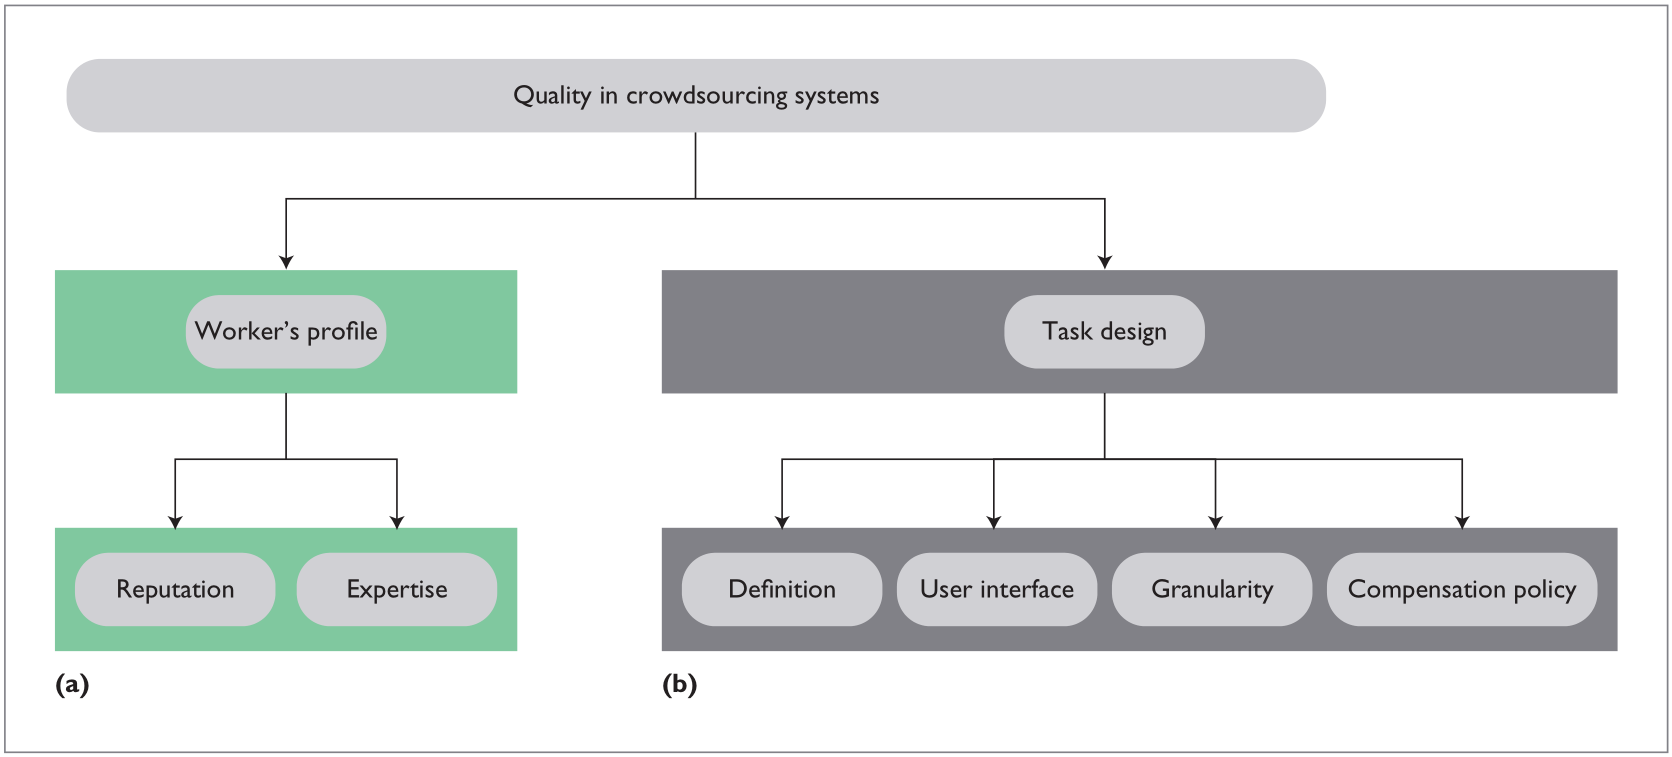
\includegraphics[width=\textwidth]{taxonomy}
		\caption{Taxonomy of quality in web-based crowdsourced systems.}
		\label{fig-taxonomy}
	\end{figure*}

	
	% Worker profiles
	%	Reputation
	%	Expertise
	% Task design
	% 	Task definition
	%	User interface
	%	Granluarity
	%	Compensation policy
	
	
	% Quality control approaches
	% Design time and runtime (see tables)
	% Why approaches are needed even for highly-skilled users
	% Requesters must specify runtime approaches
	
	\begin{figure*}
	\rowcolors{2}{gray!25}{white}
	\begin{tabularx}{\textwidth}{|XlXl|}		
		\rowcolor{gray!50}
		\hline
		Quality-control approach & Subcategories & Description & Sample application\\
		Effective task preparation & Defensive design & Provides an unambiguous description of the task; task design is defensive---that is, cheating isn't easier than doing the task; defines evaluation and compensation criteria &  \\
		Worker selection & Open to all & Allows everybody to contribute to the task & ESP Game, Threadless.com \\
										  & Reputation-based & Lets only workers with prespecified reputation levels contribute to the task & Mturk, StackOverflow \\
										  & Credential-based & Allows only workers with prespecified credentials to do the task & Wikipedia, StackOverflow \\ \hline
	\end{tabularx}
	\caption{Existing quality-control design-time approaches.}
	\label{fig-tbl1}
	\end{figure*}
	
	\begin{figure*}

		\rowcolors{2}{gray!25}{white}
		\begin{tabularx}{\textwidth}{|lXX|}
			\rowcolor{gray!50}
			\hline
			Quality-control approach & Description & Sample application \\
			Expert review & Domain experts check contribution quality. & Academic conferences and journals, Wikipedia \\
			Output agreement 		& If workers independently and simultaneously provide the same description for an input, they are deemed correct. & ESP Game \\
			Input agreement 		& Independent workers receive an input and describe it to each other.
			If they all decided that it's a same input, it's accepted as a quality answer. & Tag-A-Tune \\
			Group truth 			& Compares answers with a gold standard, such as known answers or common sense facts to check the quality. & CrowdFlower, MTurk \\
			Majority consensus 		& The judgment of a majority of reviewers on the contribution's quality is accepted as its real quality. & TurKit, Threadless.com, MTurk \\
			Contributor evaluation 	& Assesses a contribution based on the contributor's quality. & Wikipedia, Stack Overflow, MTurk \\
			Real-time support 		& Provides shepherding and support to workers in real time to help them increase contribution quality. & \\
			Workflow management 	& Designs a suitable workflow for a complex task; workflow is monitored to control quality, cost, and so on, on the fly. & \\
			 \hline
		\end{tabularx}
	\caption{Existing quality-control runtime approaches.}
	\label{fig-tbl2}
	\end{figure*}
	
	\subsection*{Ubiquitous Crowdsourcing}
	
	Thanks to the rise of smartphones, a new type of crowdsourcing has been created. Ubiquitous crowdsourcing is smartphone owners contributing data about their outside world, such as GPS location, or ambient noise level. For example, Google Maps, or Waze, both rely on crowdsourced data to give information about traffic conditions, wrecks, and other events that happen on the road. 
	
	A major issue that faces developers who wish to use ubiquitous crowdsourcing is quality control. Just like in web-based crowdsourced, the data gathered from ubiquitous applications must be controlled for quality. For ubiquitous systems, quality control is even more important than web-based systems, in a lot of cases. On top of dealing with outright malicious users submitting bad data, the "fuzziness" of the real world requires us to deal with a truly huge amount of possible edge cases. Getting usable data out of the mess is what this paper will be discussing.
	
	\begin{figure}
		\centering 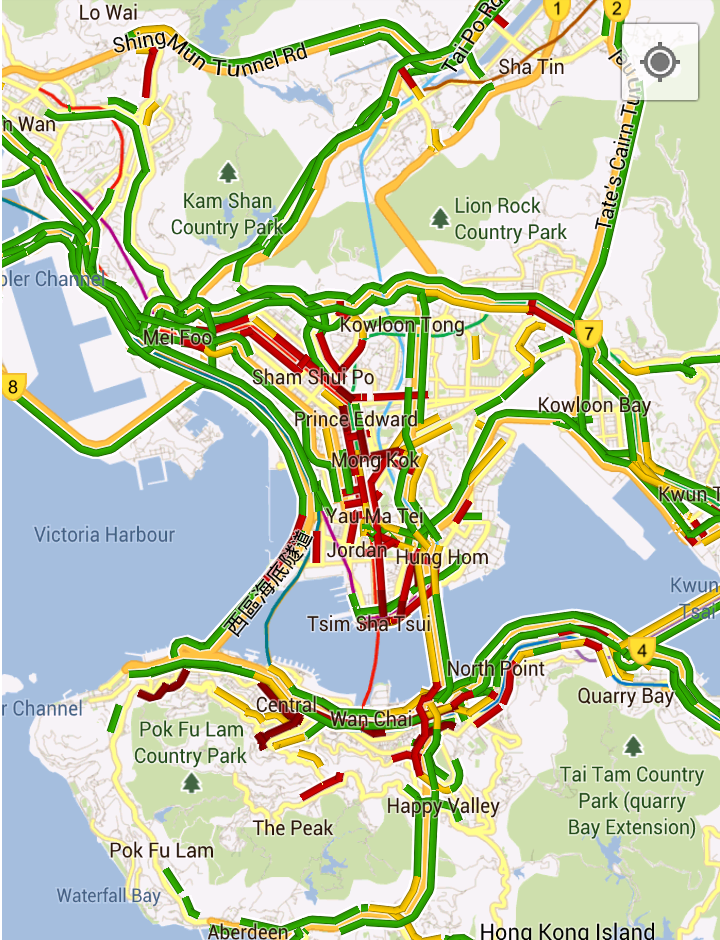
\includegraphics[width=0.7\columnwidth]{maps-traffic}
		\label{fig-traffic}
		\caption{A popular use of ubiquitous crowdsourcing: Google Maps' traffic data}
	\end{figure}

	Two other issues that ubiquitous crowdsourcing faces that web-based crowdsourcing doesn't have to deal with are Real-time Events, and Dynamic Crowds.
	\begin{itemize}
		\item \emph{Real-time Events}: ubiquitous crowdsourcing inherently deals with real-time events. The data is gathered in real time, and in many instances, real-time processing of the data is expected as well. %Example? Bus stop and location logging?
		In web-based crowdsourcing, on the other hand, quality control can often be delayed by some amount of time, if needed, to be checked and flagged by an authorized or more credible user. 
		
		
		\item \emph{Dynamic Crowds}: since ubiquitous crowdsourcing deals in real-time, the crowd itself is also often dynamic. People start and stop driving all the time, for example. The challenge of a dynamic crowd is that there are times when the number of contributors might not reach critical mass. Having too few points of data makes quality control even more important, on top of increasing the challenge of getting the proper results from the program.
	\end{itemize}
	
	Participatory sensing is the concept of communities (or other groups of people) contributing sensory information to form a body of knowledge. %\cite https://www.wilsoncenter.org/sites/default/files/participatory_sensing.pdf
	A common problem with participatory sensing is data corruption, or malicious users intentionally sending invalid or fallacious data. The paper %cite [17]
	[] shows a new concept of controlling for this by allowing consumers of the crowdsourced data to assign trust scores to specific sources of data. 
	
	The only other paper that is related to our work is []. %cite [8]
	In that paper, the authors consider the scenario where users deliberately try to confuse the sensor and send false data. The solution the authors propose is using a trust-based rating system, where each contributor has a reputation, or trust, rating and processed the data sent from users based on this rating. While their system shows an improvement over other trust-based systems, we propose an improvement to that system.
	% III. The credibility-weight and proposed approach
	%	1. Using mobility patterns
	%	2. Defining POIs via tuples
	%	3. Regularity function (how regularly a user visits a place)
	%	4. Trustworthiness score, or reputation
	%	5. Final formula and explanation
	
	Our proposed method is to track the users' mobility patterns. Studies have shown that data can be very consistent when cross-referencing with a users' commute. For example, there is a high degree of regularity in a weekday commute; most people tend to make a schedule and stick to it when traveling. [] %Cite the article [18]
	We look at taking a public bus, and users' traveling patterns to determine when the busses will arrive at given stops. First we define, for each user, Points of Interest (POIs) with tuples, $T(loc_{POI_x}, t_i)$. $loc_{POI}$ is the specific point where the contribution was submitted. $t_i$ is a logical time as opposed to a timestamp. We define a logical time as something application-relevant, such as \emph{morning}, \emph{afternoon}, or \emph{late night}.
	While processing the data, we consider patterns differently for weekdays vs. weekends, since people generally have more regular schedules on the weekdays. %Include figure?
	
	Based on this, and with this framework, we define a regularity function $Reg(T_j)$ whose values are calculated based on location readings from the users GPS.
	While there is obviously no history data from the start of the logging process, after just a few days of logging data we can begin to put together a fairly accurate regularity function for the user. We start to define POIs for the user as \emph{local}, \emph{familiar}, and \emph{stranger}. 
	
	\begin{figure}
		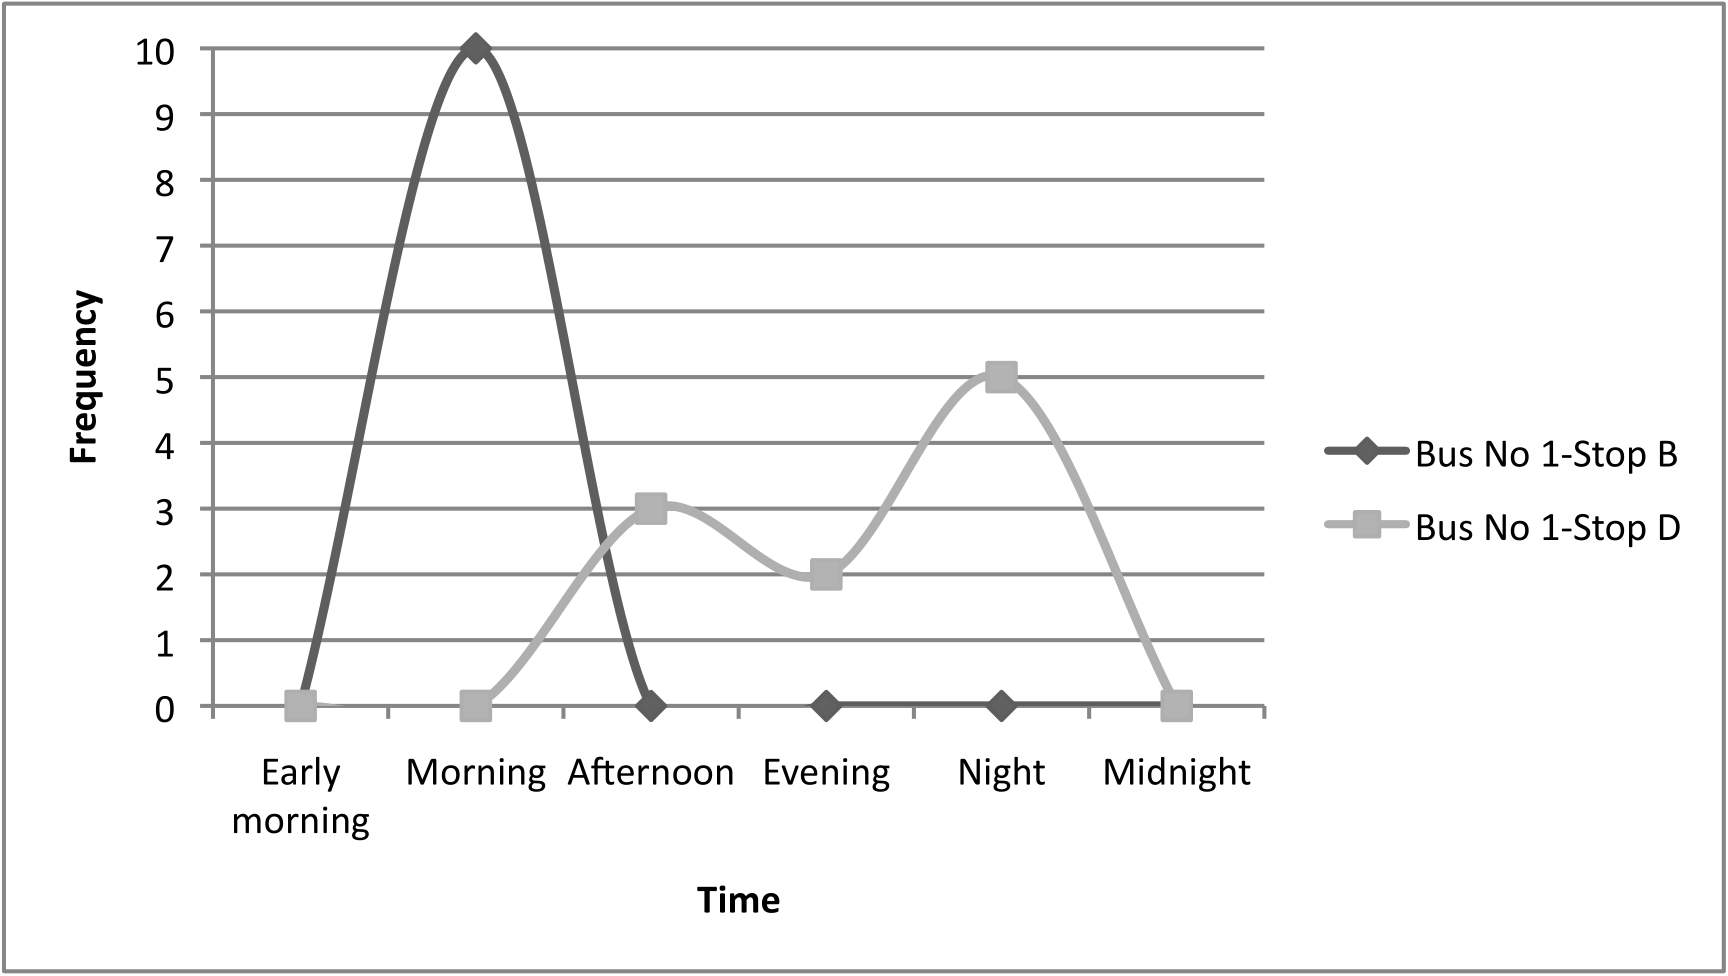
\includegraphics[width=\columnwidth]{freq-dist}
		\caption{Frequency distributions for regularity function for a given user}
		\label{fig-freq}
	\end{figure}
	
	On top of the regularity function, we also define a reputation score. When the user submits data, it is checked against other users submissions and also their own regularity function to determine a trustworthiness score, $Trust(u_i)$. For web-based crowdsourcing, this kind of trust function is usually created by reviews on the users' input from experts, but in ubiquitous crowdsourcing the rating must be different, as there is both too much data and not enough time for \'experts\' to rate each user. On top of that, using the formula we created, it is still possible to use data from locations where the user-submitted data is very sparse. Based on the regularity and trust functions, we can compute a credibility weight for user $u_i$:
	
	$$\text{credibility weight} (T_j) = $$ 
	$$\alpha \cdot Reg(T_j) + (1 - \alpha) \cdot Trust(u_i)$$
	
	$\alpha$ can be adjusted on the fly to give more weight to either the trust or regularity functions for the overall credibility weight. For example, if there is an area with a large amount of submissions, the regularity function of each user might not be as important as the trust score, and visa-versa in low-data areas.
	
	\section*{Related Works}	
	Many websites are crowdsourced-based. The most popular is Wikipedia, the entirely user-submitted encyclopedia. Wikipedia is obviously not ubiquitous crowdsourcing, rather the first type of web-based crowdsourcing/data entry we mentioned, and so has different requirements for ensuring quality control than our formula, but it is still an excellent platform to look at. Many other such platforms exist, and often they use drastically different quality control methods. StackOverflow, for example, relies on a combination of explicit user ratings and also authorized moderators to police responses and questions. It is easy to see the design time strategies versus the runtime strategies the creators of StackOverflow have put into place. 
	
	
	
	
	\section*{Conclusion}	
	We are creating an Android-based application that will give more accurate crowdsourced data about bus locations, based on the formula of this paper. We believe ubiquitous crowdsourcing has only just started to come into real force, and we want to show that its power is larger than was previously believed. Along with being powerful, we want to show the data is reliable, hopefully attracting many people to our application, giving more reliable data about bus positions. 
	
	We are paying special attention to the runtime factors of our quality control algorithms and designs. We hope our research encourages more people to develop crowdsourced applications and programs, allowing them to accurately and more easily be able to control for quality in their user submissions.
	
	\bibliography{FirstDraft}
\end{document}


